%! Author = adam
%! Date = 28.02.21

\chapter{Basics of Interactions of Ions with Matter}\label{ch:basics-of-interactions-of-ions-with-matter}
Well to put together what we have done so far: Ion Sources $\rightarrow$ accelerating those ions $\rightarrow$ transporting those ions $\rightarrow$ quantifying the important parameters of your final ion beam.

I'd say we are ready to start having these ions interact with matter!
Some keywords before we begin:

\begin{myitemize}
\item Ion penetration depth
\item sputtering
\item doping with foreign atoms
\item change of mechanical, optical, electrical, and magnetic properties
\end{myitemize}

\section{Interaction Forces in Solids and Vacuums}\label{sec:interaction-forces-in-solids-and-vaccums}
When we want to discuss how ions interact with matter, we must examine in detail the short and long range inter-atomic forces.
For the simple case, in a vacuum, we have two extrema of interaction for two particles with charges $Z_1$ and $Z_2$.
At the long range interaction, we have the Coulomb electrostatic interaction, which has a potential:
$$V_c(\vec{r}) = -\frac{Z_1 Z_2 e^2}{\vec{r}}$$
where $\vec{r}$ is the distance vector between the two.
This scales with $\propto \frac{1}{r}$, but it is important to note that this long range interaction potential exists only when both particles are charged!
On the other side, the short range interaction, we have quantum mechanic forces governing, for example the Pauli exclusion principle.
This regime in which short range applies is when atomic orbital overlap.
This interaction exists even when particles are neutral, which is not the case for the long range interaction, so these short range interactions can happen for ion-atom or atom-atom combinations.
If we turn our attention outside a vacuum, and into a solid, we have the Lennard-Jones potential as seen in Figure~\ref{fig:LJPfig}.
The reason we use this is that the voltage in a solid or crystal is normally unknown, or at least very complex, so the LJP is a nice approximation.
This potential depends on the interaction distance $\vec{r}$ and is given by:
$$V(\vec{r}) = \frac{pq}{p-q} \Delta E \left[ \frac{1}{p} \left( \frac{r_0}{r} \right)^p - \frac{1}{q} \left( \frac{r_0}{r}\right)^q \right]  $$
In this rendition of the LJP, $p$ and $q$ are fitting parameters, but the important part of this equation is $\Delta E$ which is the energy at the equilibrium atomic distance $r_0$, i.e., $\Delta E = V(r_0)$.
It can also be considered the binding energy of the atom into the solid, i.e., the energy one must apply to pull out the atom from the crystal into the free space.
If the atom is in the inter-atomic distance $r_0$, then it is in the most stable configuration of the atom in the solid.
In reality, the potential will probably look something different from that of the LJP, but it is a good model and easy to handle.
\begin{figure}
	\centering
	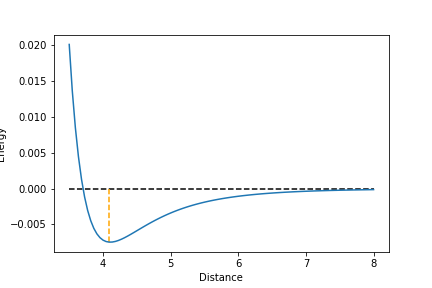
\includegraphics[width=0.6\linewidth, height=6cm]{LJP}
	\caption{The orange dashed line represents $\Delta E$, i.e., the energy at the equilibrium atomic distance $r_0$. }
	\label{fig:LJPfig}
\end{figure}

\section{Collisions of Ions with Atoms}\label{sec:collisions-of-ions-with-atoms}
Now we imagine an ion with energy $E$ flying towards a target atom.
Depending on the energy of the ion, there will be different minimum interacting distances $r$ during the scattering process.
At impact, the wave functions of the ion and atom will overlap, so it is very important to know the inter-atomic potential of the sample.
If we have a high $E$, then we have a low $r$, and with low energy ion $E$, then there will be a high $r$.
However, this is a many body problem, so we will have nuclei and electrons of the ions as well as those in the atoms factoring into the potential, which in turn will be very complex, since we must take into account the interaction of electrons and nuclei.
So we must consider realistically two reference points: the Bohr radius $a_0 = 0.5\angstrom$ and $r_0$ from the LJP (the spacing of atoms in a crystal).
If $r >> r_0$, the crystal atoms are undisturbed by the incoming ion.
When $r << a_0$ the nuclei of ion and crystal atom form the closest pair of charged particles, so the Coulomb force dominates!
At the intermediate distance $a_0 < r < r_0$, we will have electrostatic repulsion Coulomb force, but also an overlap of the electrons of the two atoms, so there is energy to promote some electrons to higher electron energy levels due to the Pauli principle.
We get a modified Coulomb potential from this, and it is called the screening potential since as the ion approaches the atom, the electron orbitals overlap and repulse each other.
The screening potential can be written as $$ V(r) = -\frac{Z_1 Z_2 e^2}{r} \chi(r)$$ with $\chi \rightarrow 0$ for $r \rightarrow \infty$ and $\chi \rightarrow 1$ for small $r$.
An important screening potential, called the universal screening potential was determined by Ziegler, Biersack and Littmark~\cite{3}.
Now that we have discussed which laws are coming into play as ions get close to a sample, we can now find out what happens afterwards.
When an ion penetrates into a sample, there will be a number of collisions that it makes with the atoms within the sample.
At some point, the ion will be tired from being scattered so much and will remain at rest.
What happens during these collisions?
We can model them as \textbf{binary elastic recoils}.
Binary is coming from the fact that we will consider just the ion and the target atom it is being deflected from its initial direction.
There are interactions with the electrons of the solid, but this will result in energy loss of the ion and not so much a proper deflection resulting from a nucleus.
There are two extrema of collisions, \textit{violent} and \textit{soft}.
Violent collisions are when the energy of the incident ion $E_i$ is equal to or larger than a few keV resulting in a small interaction distance $r$.
For soft collisions, the energy of the ion is smaller than about 1 keV. This means we have an increased $r$, and we will have no longer a two body collision, but rather multi body collisions.
The term elastic comes from the fact that if we know the initial energy of the ion, we can determine the energy change that occurred from the collision.
Enough elastic collisions and the particle will finally lay to rest (think classically!).


\section{Scattering}\label{sec:scattering}

\begin{figure}
	\centering
	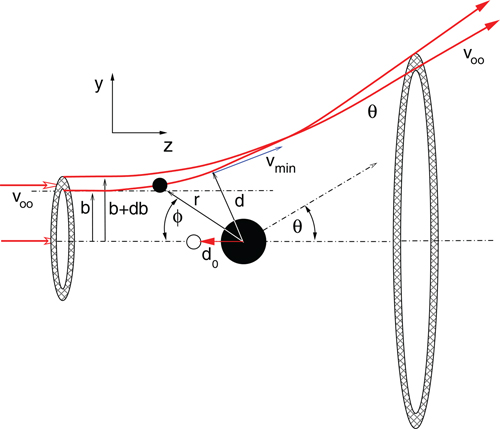
\includegraphics[width=0.6\linewidth, height = 6cm]{rutherford}
	\caption{Also know as rutherford scattering, a microscopic view of the scattering process (inside a foil for example).}
	\label{fig:rutherford}
\end{figure}
A term that may better fit than scattering cross-section, is \textit{angular differential scattering cross-section}.
We shall now try to define it.
Imagine we scattered ions through a thin foil and used at a distance $R$ away from the foil a detector with area $\Delta a$ at an angle $[\theta_c, \theta_c + \Delta \theta_c]$ where $\theta_c$ is the scattering angle of the ions that passed through the foil.
The thin foil will impact the ion with different impact parameter $b$ (this distance between the ion and the 'tangent atom', i.e., minimum interaction distance) and thus a different scattering angle.
The definition of this differential scattering cross section $dn_\theta$ is the number of ions scattered to the area $\Delta a$ (between  $[\theta_c, \theta_c + \Delta \theta_c]$) per unit time.
If $I_0$ is the flux of incident ions, the unit-less solid angle of the detector $\Delta \Omega$ is given by
$$\Delta \Omega = \frac{\Delta a}{R^2} = \frac{(R\Delta \theta_c) (R\sin\theta_c \Delta phi)}{R^2} = \Delta \theta \Delta \phi \sin\theta_c$$
The differential cross scattering would then be defined as $d\sigma (\theta_c)$ (normally in units of mm$^2$) and can be written with the help of the solid angle:
$$ \frac{d\sigma(\theta_c)}{d\Sigma} = \frac{1}{I_0} \frac{dn_\theta}{d\Omega} $$
The term on the LHS is the differential scattering cross section per unit solid angle, while on the RHS we have the inverse incident ion flux multiplied by the number of scattered ions into $[\theta_c, \theta_c + \Delta \theta_c]$ per unit solid angle and per unit time.
From Figure \ref{fig:rutherford} we see that the differential cross section can be written as $d\sigma = 2\pi b db$, thus the differential scattering cross section can be written
$$\frac{d\sigma (\theta_c)}{d\Omega} = \frac{b}{\sin\theta_c}\left|\frac{db}{d\theta_c}\right| $$
By measuring the scattering angle, we can get information of the impact parameter $b$.
So we can get really microscopic information just by measuring the scattering angle!
An important thing that happens during scattering is the transfer of energy, thus we must describe the \textit{energy transfer cross section}.
Image an ion beam with certain ion flux directed at a thin foil with target molecules.
The thickness of the foil is $\Delta x$ (extremely thin), where the area can be defined as a unit area.
Within the area you have scattering centers, the target atoms.
They can be defined as cross section areas $\sigma$.
We need a probability function to describe these scattering events dependent on the energy of the ions $E$.
We could then assume for $N$ scattering atoms per unit volume, we can calculate the number of target nuclei in our thin foil: $N \Delta x$ target nuclei (per unit area).
The total fraction of target nuclei in the surface area that act as scattering atoms is then $\sigma N \Delta x$.
All of this leads us to the probability $P$ that an ion with energy $E$ will undergo a scattering event:
$$P(E) = N\sigma(E) \Delta x$$
which can then be folowed up with the probability for transfer of energy $[T, T + dT]$ is
$$P(E, T)dT = \frac{dP(E)}{dT}dT = N \Delta x \frac{d\sigma (e)}{dT} = \frac{1}{\sigma (E)}\frac{d\sigma (E)}{dT}dT$$
The term $\frac{1}{\sigma (E)}$ is the total energy transfer cross section, and $\frac{d\sigma (E)}{dT}$ the differential energy transfer cross section.
This can be further calcualted in terms of impact parameter
$$\frac{d\sigma (E)}{dT} = \frac{4 \pi}{T_m} \frac{d\sigma (\theta_c)}{d\Omega} = \frac{4\pi}{T_m} \frac{b}{\sin\theta_c} \left| \frac{db}{d\theta_c} \right| $$
where $T_m = \frac{4m_1 m_2}{m_1 + m_2} E_u$ is the maximum transfer of energy during a scattering process.
The total cross section if the probability of impact is 1 can be calculated in terms of energy
$$\sigma (E) = \int_{T_{min}}^{T_{max}} \frac{d\sigma (E)}{dT}dT $$
or scattering angle
$$ \sigma (\theta_c) = \int_{b_{max}}^0 \frac{d\sigma (\theta_c)}{db}db =  \int_{b_{max}}^0  2\pi b db $$
but both are equivalent.
So that was a lot of basics for the understanding of ions in solids, and now we will actually apply this knowledge to calculate what will be the energy transfer during a whole path, what will be the damage, and ion energy range.

\section{Summary}\label{sec:summary3}

\begin{myitemize}
	\item samples have difficult potentials, so we can approximate using the leonard jones potential
	\item Depending on the energy of an ion, the interaction distance $r$ will change.
	For high $E$, we have low $r$, and vice versa for low $E$.
	\item Screening potential comes from the combination of Coulomb force with the Pauli exclusion principle at short distances, and the universal screening potential was discovered by Ziegler
	\item  Scattering is complicated but draw a picture and it should be fine.
    By measuring the scattering angle, we can determine microscopic properties of the interaction ($b$)
\end{myitemize}
